\section{Action Figure Nodes}

The AO network provides decentralization and security by incentivizing diverse participants to participate as node operators

\begin{figure}[h]
  \centering
  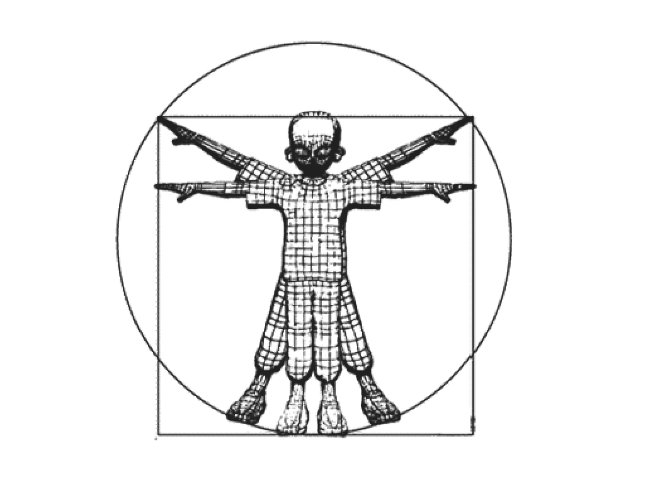
\includegraphics[width=\columnwidth]{images/image12.png}
  \caption{None of them are as strong as all of us: Connecting Action Figures to node operation at the UI level makes node operation more accessible, helps decentralize the Action substrate, and improves network security}
  \label{fig:action_figure_nodes}
\end{figure}

The Action substrate, leveraging AO's network, may further incentivize security and sovereignty by tying hyperobjects to validated node operation:

\begin{itemize}
\item Action's directional strategy is to eventually evolve to operate its own compute, with Action Figures (and potentially other hyperobjects) functioning as nodes
\item Nodes on AO can be customizable with devices and WebAssembly and can integrate with other services via relay device. Nodes on Action may be customized in certain ways, e.g. optimized for inference\footnote{Inference optimization would involve configuring nodes with optimizations (hardware and/or software) for AI/ML tasks. This includes using techniques like model quantization, parallel processing, and hardware acceleration to improve the performance of inference in processes.}
\item Broadside OGs will be the first Action Figures equipped with node functionality in our first experiments with this idea
\item By making Action Figures function as a 'front end' for nodes \ref{fig:action_figure_nodes}, node operation becomes more accessible to a larger cohort of users
\item Growing this community strengthens the security of the network
\end{itemize}
